\documentclass{article}
\usepackage[german]{babel}
\usepackage{float}
\usepackage{fourier}
\usepackage[utf8]{inputenc}
\usepackage[T1]{fontenc}
\usepackage{amsfonts,amsthm, amsmath}
\usepackage{listings}
% The following is needed in order to make the code compatible
% with both latex/dvips and pdflatex.
\ifx\pdftexversion\undefined
\usepackage[dvips]{graphicx}
\else
\usepackage[pdftex]{graphicx}
\DeclareGraphicsRule{*}{mps}{*}{}
\fi

\setlength\parindent{0pt}
\lstset{language=Java}

\begin{document}

\textbf{Team:} TEAM 01, Falco Winkler (FW), Daniel Schruhl (DS)\\
\\
\textbf{Aufgabenteilung:}
\begin{itemize}
    \item IDL Compiler
    \item Namensdienst
    \item mware\_lib Library
\end{itemize}

\textbf{Quellenangaben:}
\begin{itemize}
    \item Aufgabe 4, 11.06.2017, C. Klauck \& H. Schulz: \newline
    http://users.informatik.haw-hamburg.de/~schulz/pub/Verteilte-Systeme/AI5-VSP/Aufgabe4/
\end{itemize}

\textbf{Bearbeitungszeitraum:}
\begin{itemize}
	\item 11.06.2017 4 Stunden (DS)
\end{itemize}

\textbf{Aktueller Stand:}
\begin{itemize}
	\item IDL Compiler begonnen
    \item Namensdienst
    \item mware\_lib Library
\end{itemize}

\textbf{Änderung des Entwurfs:}
\begin{itemize}
    \item Keine Änderungen
\end{itemize}

\newpage

\section{Einführung und Ziele}
Es soll eine einfache objektorientierte Middleware entworfen werden, die Methodenaufrufe
eines entfernten Objektes ermöglicht.

Zur Orientierung gilt hierbei die CORBA Architektur. Genauer soll hier ein ORB zur
Verfügung gestellt werden, der es ermöglicht Methoden von entfernten Objekten aufzurufen.

Zur Abstraktion und Beschreibung der Schnittstellen der Objekte soll eine IDL verwendet werden.
Diese IDL wird dann zur Erzeugung von Klassen- und Methodenrümpfen verwendet.

Außerdem beinhaltet der ORB einen Namensdienst, der Objektreferenzen in einem Netz mit Namen finden
kann.

Die Middleware an sich soll durch eine Library abstrahiert und verwendbar sein.

\subsection{Randbedingungen}
Der Namensdienst soll auf einem entfernten Rechner unabhängig von der Middleware Library
lauffähig sein. Der Port muss zur Laufzeit einstellbar sein.

Der IDL-Compiler soll in einem Package oder einer \texttt{.jar} Datei zur Verfügung gestellt
werden. Der Compiler soll folgende IDL Typen unterstützen:

\begin{itemize}
    \item module (keine Schachtelung, 1 Modul pro Datei)
    \item class (nicht als Parameter oder Returnwert, keine Schachtelung)
    \item int
    \item double
    \item string
\end{itemize}

Ein Beispiel:
\begin{lstlisting}
module math_ops {
  class Calculator {
   double add(double a, double b);
   string getStr(double a);
 };
};
\end{lstlisting}

Die Middleware Library soll in einem Package \texttt{mware\_lib} zusammengefasst werden.

Wenn eine Serverapplikation während eines entfernten Methodenaufrufes eine RuntimeException
wirft, soll diese an den Aufrufer weitergeleitet werden.

Es soll möglich sein, dass zwei oder mehrere Klienten die selbe Objektreferenz zeitgleich
nutzen wollen. Das soll innerhalb der Middleware nicht zu Deadlocks führen.

\subsection{Kontextbegrenzung}
Die Implementierung soll in Java vorliegen.

Die Behebung von Deadlocks in den Anwendungen ist nicht Aufgabe der Middleware.

\newpage

\section{Gesamtsystem}
Das Gesamtsystem besteht aus drei Subsystemen, die unabhängig voneinander lauffähig sind.
Dabei sind das NameService System und das IDL-Compiler System Applikationen, die über
die Kommandozeile gestartet werden können.

Die Middleware Library (mware\_lib) ist eine Bibliothek, die in der jeweiligen Applikation,
die die Middleware verwenden soll eingebunden werden muss. Die Middleware Library ist also
nicht direkt über die Kommandozeile startbar.

\subsection{Bausteinsicht}
%\begin{figure}[H]
%    \centering
%    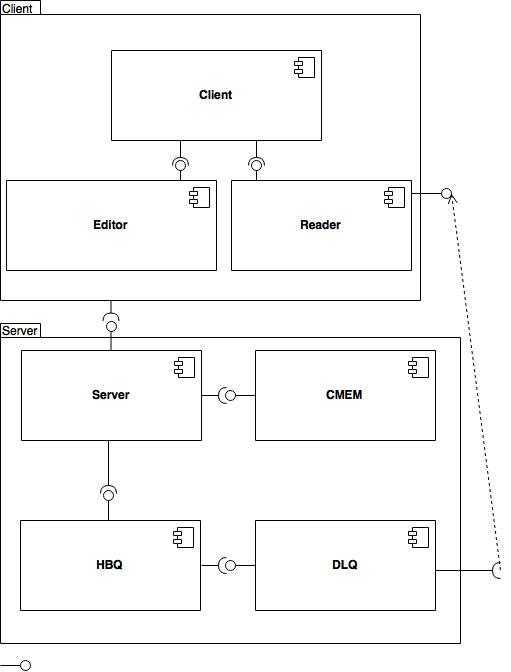
\includegraphics[width=0.5\textwidth]{component-diagram.png}
%    \caption[seq-dia]{Komponentendiagramm der Middleware Infrastruktur}
%    \label{fig:component-diagram}
%\end{figure}

\subsection{Laufzeitsicht}
%\begin{figure}[H]
%    \centering
%    \includegraphics[width=1.0\textwidth]{sequence-diagram.png}
%    \caption[seq-dia]{Eine ggT Berechnung mit Abbruch per Voting}
%    \label{fig:seq-diagram}
%\end{figure}

\newpage

\section{Subsysteme und Komponenten}

\subsection{NameService}
\subsubsection{Aufgabe und Verantwortung}
Der NameService bildet Namen auf Objektreferenzen ab. Er wird verwendet, um Objekte anhand
ihres Namens zu finden und anzusprechen und um Objekte anzumelden.

\subsubsection{Schnittstelle}
\begin{lstlisting}
Die Schnittstellen sind ansprechbar mittels u.g. Nachrichtenformat per TCP an gegebenem Port. 
public void rebind(Object servant, String name); 
Bindet ein Objekt an einen Platzhalter im Namensdienst.
public Object resolve(String name); 
Loest eine Namensreferenz auf ein Java - Objekt auf.
Das Ergebnis wird als serialisiertes Java - Objekt per TCP an den Aufrufer gesendet.
\end{lstlisting}

\subsubsection{Entwurfsentscheidungen}
Der Port, an dem der NameService läuft ist zur Laufzeit einstellbar. Das geschieht über
den Startparameter.

Der Nameservice Empfängt Nachrichten im folgenden Format:
\begin{itemize}
\item Byte 0: Art des Befehls. (0 = Rebind, 1 = Resolve, 2 = Shutdown) 
\item Byte 1 - 11: Alias für rebind / resolve
\item Byte 12 - n: Serialisiertes Objekt
\end{itemize}

\subsubsection{Konfigurationsparameter}
\begin{itemize}
    \item Port des NameServices
\end{itemize}

\subsection{IDL Compiler}
\subsubsection{Aufgabe und Verantwortung}
Der IDL Compiler hat die Aufgabe, eine gegebene Modulbeschreibung aus einer Datei
im .idl - Format einzulesen und die der Beschreibung entsprechende abstrakte Java-Klasse 
als Java-Code zu generieren. Die generierte Klasse wird auf Client und Serverseite eingebunden
und zu einer konkreten Klasse abgeleitet. Instanzen davon werden als Proxy - Objekte
für CORBA - Aufrufe verwendet.


\subsubsection{Schnittstelle}
\begin{lstlisting}
Compiler.main(String[] args)
Ueber die main - Methode der Klasse Compiler kann der Compiler ausgefuehrt werden.
Als erstes Argument muss der Pfad der .idl-Datei, als zweites Argument der Pfad zur 
Ausgabedatei angegeben werden.
\end{lstlisting}

\subsubsection{Entwurfsentscheidungen}
Die Methoden zur Übersetzung der IDL - Beschreibung werden abstrakt in einem Interface 
definiert. Die Eigentliche Übersetzung nimmt IDLToJavaTranslator (die Implementierung des 
Interfaces) vor. So ist der Übersetzungsprozess logisch von der Syntax der zu übersetzenden
Sprache getrennt, und die Testbarkeit der einzelnen Vorgänge gegeben.
\subsubsection{Konfigurationsparameter}

\begin{itemize}
    \item Pfad zur Eingabedatei
    \item Pfad zur Ausgabedatei (existierende Dateien werden überschrieben)    
\end{itemize}

\end{document}